% ============================================================================
% Hyper-Relational KG vs In-Context LLM Reading: Where Does the Bottleneck Lie?
% A Production-Realistic Evaluation on the Bank of Korea Compensation Regulations
% ============================================================================
% Target: ISWC 2026 In-Use Track (Springer LNCS, ~16 pages)
%
% Build:
%   xelatex main && bibtex main && xelatex main && xelatex main
% (XeLaTeX needed for kotex Korean rendering of inline domain examples.)
%
% NOTE: This skeleton uses the standard \documentclass{article} for portability.
% When migrating to the official LNCS template, replace the class line with
%   \documentclass[runningheads]{llncs}
% and drop article-only packages (geometry, fancyhdr) that LNCS overrides.
% ============================================================================

\documentclass[11pt,a4paper]{article}

% --- Geometry / typography ---
\usepackage[margin=2.5cm]{geometry}
\usepackage{microtype}

% --- Korean (XeLaTeX + kotex). Comment out if compiling with pdflatex. ---
\usepackage{kotex}

% --- Math, symbols ---
\usepackage{amsmath,amssymb}

% --- Tables ---
\usepackage{booktabs}
\usepackage{multirow}
\usepackage{array}

% --- Graphics / TikZ ---
\usepackage{graphicx}
\usepackage{tikz}
\usepackage{pgfplots}
\pgfplotsset{compat=1.18}
\usepackage{pgfplotstable}

% --- Cross-refs / hyperlinks ---
\usepackage[hidelinks]{hyperref}
\usepackage{cleveref}

% --- Bibliography (LNCS uses splncs04.bst; for now use plain numeric) ---
\usepackage[numbers,sort&compress]{natbib}

% --- Custom commands ---
\newcommand{\krw}[1]{#1\,KRW}
\newcommand{\backendname}[1]{\texttt{#1}}

\title{Where Does the KG-RAG Bottleneck Lie?\\
A Production-Realistic Evaluation of Hyper-Relational Knowledge Graphs vs.\
In-Context Surface Forms}

\author{Yongmin Kim\thanks{NAVER Corp.}\\
\texttt{kim.yongmin@navercorp.com}}

\date{\today}

\begin{document}

\maketitle

\begin{abstract}
We evaluate a production-deployed retrieval-augmented question-answering
system over the Bank of Korea Compensation Regulations on a 100-question
benchmark spanning ten categories and four large language model
families. The system fields four backends — a hyper-relational
knowledge graph (TypeDB v3), a property graph (Neo4j), a preprocessed
context retriever, and a closed-book baseline — alongside four
in-context surface forms in which the entire knowledge graph is dumped
into the prompt as TypeQL, Cypher, JSON-LD, or natural language.
Counterintuitively, the production knowledge-graph agents underperform
the in-context surface forms by 21--30 percentage points on multi-key
queries (paired McNemar $p<0.05$ in 5 of 8 comparisons), despite the
agents having strictly more data. Disentangling \emph{query generation}
from \emph{KG expressivity}, we find that natural-language summary of
the same KG facts is Pareto-optimal in the (accuracy, token cost)
frontier (88.75\% mean accuracy, 14K vs 32K characters), and that one
LLM family (Llama-4-Scout) exhibits a 21-percentage-point form
sensitivity that other families do not — directly tracing the bottleneck
to query-language familiarity rather than KG expressivity. We further
show that in-context KG dumps are paradoxically weaker than natural
language at \emph{closed-world boundary inference} (proving absence),
because the schema-driven structural clarity of the KG is stripped when
serialized as a raw dump. We argue that KG infrastructure should be
valued as the \emph{operational backbone} of the system rather than as
the LLM-facing surface form, and propose explicit boundary annotations
in KG-to-natural-language conversion pipelines as a practical remedy.
\end{abstract}


\section{Introduction}\label{sec:intro}

Production retrieval-augmented question-answering systems are
increasingly built on top of knowledge graphs (KGs). For domains where
facts are inherently multi-relational — public-sector regulations,
clinical guidelines, organizational policies — the canonical argument
for a KG backbone runs as follows. Natural-language documents lose
the schema-driven structure that the regulation \emph{has} as a fact
base. A binary triple store flattens N-ary relations and forces
either lossy decomposition or awkward reification. A
hyper-relational KG (e.g., TypeDB v3) preserves the original role-
player structure faithfully, and a ReAct-style agent can in principle
exploit that structure via formal queries (TypeQL, Cypher) for
multi-hop reasoning.

\paragraph{Scope.} Our setting is a regulatory KG-RAG deployment in
which the entire structured fact base fits within a modern LLM's
32K-token context window. We argue this scope is unusually broad in
practice: regulations, organizational policies, clinical guidelines,
benefits schedules, and many similar enterprise corpora have fact
bases of low single-digit megabytes once serialized, well below
state-of-the-art context limits. The claims in this paper are
explicitly scoped to such fact-bounded domains; multi-million-fact
KGs (knowledge bases of the open Web, biomedical corpora, etc.)
require retrieval and are out of scope for the surface-form ablation.

This paper reports a counterintuitive finding from a production
deployment of exactly such a fact-bounded system. Over the Bank of
Korea Compensation Regulations — a 200-page Korean public-sector
document with eight N-ary fact tables and twelve supplementary
clauses — we evaluate four LLM families against eight backends (TypeDB
hyper-relational agent, Neo4j property-graph agent, production
chunked-context retriever, closed-book LLM, and four
\emph{in-context surface-form} variants in which the entire KG is
serialized into the prompt as TypeQL, Cypher, JSON-LD, or natural
language). The benchmark is 100 questions covering ten categories,
including 42 multi-key questions that stress the supposed strength
of the hyper-relational KG.

The headline result is that the production KG agents
\emph{underperform} every in-context surface form by 8--26
percentage points (paired McNemar $p<0.05$ in 5 of 8 KG-vs-context
comparisons). Three observations make this counterintuitive:
(i) the KG agents have access to \emph{strictly more facts} than
the in-context dumps; (ii) the gap is largest exactly in the
multi-key categories that the KG was designed to serve; and
(iii) the closed-book baseline is at 9--13\%, ruling out
pre-training memorization as the explanation.

The surface-form ablation localizes the bottleneck. Four findings
result.

\begin{enumerate}
\item \textbf{The query-generation stage, not KG expressivity, is
      the dominant accuracy determinant.} An in-context dump with
      the same hyper-relational structure as the KG store reaches
      83--95\% accuracy across LLMs, while the production agent
      built on top of the KG reaches 56--73\%. The 8--26 percentage
      points lost between the two are absorbed by the agent's
      query-authoring, query-execution, and result-verbalization
      stages.
\item \textbf{Natural-language summary Pareto-dominates structured
      surface forms.} Across LLMs, NL achieves a mean accuracy of
      89.8\% at 14K characters, beating the structured tiers
      (TQL/Cypher/JSON-LD) at 83--85\% and 26--32K characters.
\item \textbf{Llama-4-Scout exhibits a 21-percentage-point form
      sensitivity that other LLMs do not.} The asymmetry traces to
      query-language familiarity in pre-training, with single-fact
      lookups surviving unfamiliar syntax but cross-reference tasks
      collapsing — a finding directly testable via guide ablation.
\item \textbf{In-context KG paradoxically underperforms NL on
      closed-world boundary inference.} The structural strength of
      the KG (schema-driven clarity, integrity rules) is stripped
      away when serialized; the resulting raw dump leaves the LLM
      to enumerate-and-disprove rather than read an explicit
      boundary clause.
\end{enumerate}

We argue for a reframing of KG infrastructure value: the KG should
be treated as the \emph{operational backbone} of the system —
schema enforcement, multi-system integration, latent expressivity
for stronger query agents — rather than as the LLM-facing surface
form. As a practical recommendation, we propose adding a
KG-to-natural-language conversion layer between the KG store and
the LLM, augmented with explicit boundary annotations to address
the closed-world inference gap. Section~\ref{sec:discussion}
develops these implications.

\subsection*{Contributions}

\begin{itemize}
\item We report the first production-deployment evaluation of
      TypeDB v3 hyper-relational and Neo4j property-graph KGs
      against a four-tier in-context surface-form ablation
      (Section~\ref{sec:results}).
\item We demonstrate that the query-generation stage is the
      dominant accuracy bottleneck in current KG-RAG agents,
      not KG expressivity (Section~\ref{sec:results}).
\item We identify and decompose two distinct surface-form
      mechanisms — query-language familiarity and closed-world
      boundary inference — and show that they require distinct
      remedies (Section~\ref{sec:mechanism}).
\item We articulate the \emph{KG semantic paradox} and recommend
      a KG-to-NL conversion layer as the practical next step for
      KG-LLM pipelines (Section~\ref{sec:discussion}).
\end{itemize}

\section{Related Work}\label{sec:related}

\paragraph{KG-augmented retrieval.}
GraphRAG~\citep{edge2024graphrag} introduced a community-detection
approach in which a KG is constructed and then summarized at
multiple levels of abstraction; query-time retrieval selects
community summaries rather than raw triples.
HippoRAG~\citep{gutierrez2024hipporag} treats retrieval as
personalized PageRank over a KG built from a corpus, mimicking
hippocampal indexing for multi-hop QA. Both approaches construct
the KG \emph{from} the corpus; we instead start from a
production-curated KG and ask how its \emph{surface form} affects
LLM downstream accuracy. The two strands of work are complementary:
GraphRAG/HippoRAG focus on \emph{retrieval} from KGs, while we
focus on \emph{serialization} of an already-retrieved (or
in-context-feasible) KG to the LLM.

\paragraph{KG verbalization and seq2seq.}
KGT5~\citep{saxena2022kgt5} casts KG completion and KGQA as a
text-to-text task, demonstrating that LLMs trained on linearized
KGs can perform multi-hop reasoning. Our setting differs in two
ways: we use general-purpose chat LLMs (no KG-specific training)
and we evaluate \emph{multiple} surface forms head-to-head on the
same facts.

\paragraph{Hyper-relational KGs.}
StarE~\citep{galkin2020stare} provides a message-passing approach
for hyper-relational KGs, demonstrating that qualifier-augmented
relations carry information that binary-triple embeddings lose.
Earlier foundational work includes m-TransH~\citep{wen2016mtransh}
and NaLP~\citep{guan2019nalp} on n-ary relational data. These
papers establish that hyper-relational structure is real and
exploitable for embedding-based tasks. Our finding does not
contradict this: in-context LLMs handle the same hyper-relational
structure (C-TQL preserves role players verbatim) just as well
as flatter forms; the issue is not whether structure can be
exploited but whether the LLM-facing surface form is the right
place to expose it.

\paragraph{In-context behavior of LLMs.}
\emph{Lost in the middle}~\citep{liu2023lostmiddle} documents
LLMs' positional sensitivity within long contexts. While our
results do not directly engage this finding (our dumps fit
comfortably under 32K characters), it reinforces the case that
in-context surface form interacts with model behavior in
non-obvious ways. Surface-form effects in retrieval-augmented
settings are otherwise under-studied; we are not aware of prior
systematic comparisons of TQL/Cypher/NL/JSON-LD on the same
underlying facts.

\paragraph{Closed-world reasoning.}
The closed-world assumption \citep{reiter1978cwa} is foundational
in knowledge representation. Our finding that in-context KG dumps
strip closed-world semantics is, in spirit, a re-statement of
Reiter's distinction in the LLM era: \emph{absence in the dump
does not entail absence in the world}, and the LLM has no syntactic
cue to make the closure. To our knowledge, this paper is the first
to empirically measure the resulting accuracy gap between formal
KG dumps and natural-language summaries on the same out-of-scope
queries.

\paragraph{KG surveys and TypeDB.}
Hogan et al.~\citep{hogan2021kgsurvey} provide a comprehensive
survey of knowledge graphs that situates hyper-relational
representation within broader KR. TypeDB v3's TypeQL language is
documented industrially~\citep{vaticle2023typeql}; to our
knowledge, no peer-reviewed paper has evaluated TypeDB v3 in a
production LLM-agent deployment.

\section{Production System}\label{sec:system}

The system under evaluation is a deployed retrieval-augmented agent
serving compensation-policy questions over the Bank of Korea
Compensation Regulations. We summarize the architecture as it informs
our evaluation choices.

\subsection{Three Storage Backbones}

The same set of facts is materialized in three forms.

\paragraph{TypeDB v3 (hyper-relational graph).} The entire fact base
is loaded as a TypeQL ontology with N-ary relations and explicit
roles. A position-pay fact, for example, is stored as a single
relation \texttt{(해당직급:\$g, 해당직위:\$p, 적용기준:\$ref) isa
직책급결정}, in which the (job-grade, position, position-pay-amount)
triple co-participate in one fact rather than being decomposed into
binary edges. The schema (\texttt{schema/compensation\_regulation.tql})
defines 17 entity types, 8 N-ary relation types, and 35 attributes.

\paragraph{Neo4j (property graph).} The same data is loaded as a Neo4j
property graph in which N-ary relations are flattened: each
hyper-relational role-player tuple becomes a binary edge with extra
properties on the edge or on intermediate nodes. The Neo4j store has
9 node labels (e.g., \texttt{JobGrade}, \texttt{PositionPay},
\texttt{OverseasPay}) and 7 relationship types
(\texttt{HAS\_BASE\_SALARY}, \texttt{HAS\_POSITION\_PAY}, etc.).

\paragraph{Preprocessed context document.} A markdown
\texttt{regulation\_context.md} consolidates the article text (제2조
through 제15조), term-normalization rules (e.g., \texttt{G5 =
종합기획직원 5급}), calculation formulas, and four JSON lookup blocks
(salary differential, position pay, overseas salary, salary table).
This document is the input to the \backendname{context} backend,
which performs production-style chunked retrieval before invoking
the chat LLM.

\subsection{ReAct Agent}

The KG agents (\backendname{typedb} and \backendname{neo4j}) are
LangGraph state machines following a ReAct pattern. A typical step
proceeds:

\begin{enumerate}
\item The chat model receives the user question and a schema
      summary, and decides whether a database query is needed.
\item If a query is needed, control passes to the query model, which
      authors a TypeQL or Cypher query against the loaded schema.
\item The query is executed; results return as structured rows.
\item The chat model verbalizes the results into a natural-language
      answer, optionally citing schema rules.
\end{enumerate}

A failed parse triggers retry with the parse error fed back into the
prompt; the agent budget is capped at three query attempts per
question.

\subsection{Decoupled Query Agent (Setting B)}

The production code separates the chat model
(\texttt{create\_chat\_model()}) from the query model
(\texttt{create\_qwen\_model()}) by design: the original deployment
uses Qwen-Coder for query authoring even when the chat model is HCX.
For our evaluation we honour this separation by holding the query
model fixed at \texttt{Qwen3-Coder-30B-A3B-Instruct} and varying only
the chat model.

This decoupling matters: a pilot in which the same LLM played both
roles produced highly asymmetric results across LLM families,
confounding the KG vs.\ context comparison. The pilot is reported as
Setting A in Appendix~\ref{sec:appendix}; all main numbers in this
paper are Setting B.

\subsection{In-Context Surface-Form Tiers}

To isolate the contribution of the query-generation stage from the
intrinsic readability of the KG, we add four in-context backends that
side-step the agent entirely. Each constructs a single fixed prompt
of the form

\begin{quote}\small
\texttt{[article-text prefix common to all tiers]} \\[2pt]
\texttt{=== 자료 시작 ===} \\
\texttt{[KG dump in tier-specific surface form]} \\
\texttt{=== 자료 끝 ===}
\end{quote}

and invokes the chat model with this prompt as the system message and
the user question as the user message. The four surface forms (TQL,
Cypher, NL, JSON-LD) are produced from the same underlying source
tables (\texttt{eval/dump\_context\_tiers.py}), so any difference in
accuracy between tiers is purely a surface-form effect.

\section{Evaluation Setup}\label{sec:setup}

\subsection{Domain and Knowledge Source}

The evaluation domain is the Bank of Korea Compensation Regulations
(\emph{보수규정 전문, 2025-02-13 revision}), a publicly available
governance document of approximately 200 pages covering job grades,
positions, salary tables (별표 1--9), evaluation-tier differentials,
overseas pay, wage-peak schedules, and supplementary clauses (부칙).
The document mixes prose articles (제2조 definitions, 제5조 step
increments, 제9조 overtime, etc.) with multiple multi-key lookup tables.
It is small enough that the entire structured-fact set fits within a
32K-token context window, yet rich enough to expose multi-hop and
boundary reasoning.

\subsection{Question Set}

We construct a 100-question evaluation set in two stages. Thirty seed
questions were authored manually with verified gold answers traced to
the original document. Seventy additional questions were generated by
walking the underlying lookup tables with category-specific templates
(\texttt{eval/gen\_questions.py}), with weighted emphasis on multi-key
categories that stress the H1 hypothesis. The final distribution is
shown in Table~\ref{tab:eval-set}.

% Table: Evaluation set distribution (10 categories x 100 questions).
\begin{table}[t]
\centering
\caption{Evaluation set: 100 questions across ten categories. Multi-key
categories (calculation, comparison, multihop\_3key) total 42 questions
to ensure statistical power for the H1 comparison.}
\label{tab:eval-set}
\small
\begin{tabular}{l r r r}
\toprule
Category & Seed & Auto-expanded & Total \\
\midrule
single\_lookup        & 3 & 7 & 10 \\
join\_2key            & 3 & 7 & 10 \\
\textbf{multihop\_3key} & 3 & 12 & \textbf{15} \\
\textbf{calculation}    & 4 & 10 & \textbf{14} \\
\textbf{comparison}     & 3 & 10 & \textbf{13} \\
aggregation           & 3 & 7 & 10 \\
article\_text         & 3 & 5 & 8 \\
negation\_exception   & 3 & 5 & 8 \\
out\_of\_scope        & 2 & 4 & 6 \\
term\_normalization   & 3 & 3 & 6 \\
\midrule
\textbf{Total}        & \textbf{30} & \textbf{70} & \textbf{100} \\
\bottomrule
\end{tabular}
\end{table}


Each question carries a deterministic gold answer, an evidence pointer
to the source table or article, and a \texttt{required\_keys} list (a
proxy for join arity). Categories include single-key lookups
(\texttt{single\_lookup}), 2- and 3-key joins, calculations requiring
both lookup and arithmetic, comparisons across rows, aggregations,
exception clauses (negation), out-of-scope queries (combinations not
present in any table), and pure article-text questions.

\subsection{Backends}

We evaluate eight backends grouped into three classes:

\paragraph{Production agents.} The \backendname{typedb} and
\backendname{neo4j} backends invoke the production retrieval-augmented
agent: a LangGraph ReAct state machine in which a chat model performs
reasoning while a separate query model generates TypeQL or Cypher
queries against a live database. The \backendname{context} backend
uses production's chunked retrieval over a preprocessed regulation
document. We refer to this same backend as \backendname{C-MD} in the
surface-form Pareto comparison (Table~\ref{tab:token-cost} and
Figure~\ref{fig:pareto}), where it is the chunked-retrieval baseline
against the four full-dump in-context tiers. \backendname{closed\_book}
is the chat model with no retrieval — a baseline for measuring
pre-training leakage.

\paragraph{In-context surface-form ablation.} The remaining four
backends — \backendname{C-TQL}, \backendname{C-Cypher},
\backendname{C-NL}, and \backendname{C-JSONLD} — feed the \emph{entire}
knowledge graph to the chat model as a single in-context prompt, with
the only variable being the surface form. This decouples the
contribution of the query-generation stage from the in-context
reading capacity of the LLM. All four share the same article-text
prefix (the prose portion of the production context document) and
differ only in the structured-data section: TypeQL \texttt{insert}
statements (32{,}436 chars), Cypher \texttt{CREATE} statements
(32{,}030 chars), natural-language sentences (14{,}000 chars), or
JSON-LD-style nested objects (26{,}278 chars).

\subsection{Setting B: Decoupled Query Agent}

Pilot experiments revealed that when a single LLM serves both as
reasoner and as query generator, the KG agent's accuracy is dominated
by the LLM's TypeQL/Cypher syntax familiarity rather than by KG
expressivity. To remove this confound, all main experiments use
\emph{Setting B}: the chat model varies across the four LLM families
under test, while the query model is fixed to
\texttt{Qwen3-Coder-30B-A3B-Instruct}, a specialized code-generation
model that was the strongest available coder LLM in our gateway.
Production's \texttt{create\_chat\_model()} and
\texttt{create\_qwen\_model()} factories, originally designed for this
separation, are wired through environment variables.

\subsection{LLM Families}

Four LLM families serve as chat (reasoning) models. All are accessed
through a single OpenAI-compatible gateway with identical inference
parameters (temperature 0, no reasoning-mode flags); only the model
identifier varies.

\begin{itemize}
\item \textbf{HyperCLOVA X SEED-32B-Think-Text} — Korean-specialist
      think-mode model from NAVER. We confirm that without explicit
      reasoning-flag activation, no \texttt{<think>} traces appear in
      responses; HCX runs in non-reasoning mode for parity.
\item \textbf{Qwen3-235B-A22B-Instruct-2507-FP8} — frontier MoE
      instruct model from Alibaba (235B parameters, 22B active).
\item \textbf{Llama-4-Scout-17B-16E-Instruct} — Meta open-weight
      Western frontier (17B$\times$16 expert MoE).
\item \textbf{gpt-oss-120b} — OpenAI's 2025 open-weight release,
      serving as a stand-in for the closed GPT-4 family.
\end{itemize}

The query model (Qwen3-Coder-30B) is held constant across all KG-agent
runs.

\subsection{Metrics}

\paragraph{Per-item correctness.} Our scorer (\texttt{eval/scorer.py},
stdlib-only) handles seven gold-answer types: monetary amounts (with
currency and period), numbers, ratios (allowing percentage form),
booleans, sets, strings (with aliases), and refusals. For monetary
answers the scorer compares the closest numeric token in the
prediction against the gold value and verifies currency.

\paragraph{Aggregate metrics.}
For each (backend, LLM) pair we report point accuracy, the 95\%
percentile-bootstrap confidence interval (2{,}000 resamples), and a
paired McNemar exact two-sided binomial test on discordant pairs
against the relevant baseline (typically \backendname{context} or
\backendname{closed\_book}). All tests are paired by question id.

\paragraph{Surface-form size.} For the in-context surface forms, we
report the literal character count of the dump (the same string fed
to every prompt). Token cost scales roughly linearly with character
count for these largely numeric, semi-structured texts.

\section{Main Results}\label{sec:results}

% Table: Overall accuracy across 4 LLM families × 8 backends.
% n = 100 questions. Bracketed numbers are 95% bootstrap confidence intervals
% (2,000 resamples).
\begin{table}[t]
\centering
\caption{Overall accuracy on 100 questions across four LLM families and eight
backends. Bracketed values are 95\% bootstrap confidence intervals
(2{,}000 resamples). Bold marks the best in-context surface form per LLM;
italics mark the best KG agent.}
\label{tab:overall-acc}
\small
\setlength{\tabcolsep}{4pt}
\begin{tabular}{l rrrr}
\toprule
Backend & HCX-32B-Think & Qwen3-235B & Llama-4-Scout & gpt-oss-120b \\
\midrule
\multicolumn{5}{l}{\emph{Production KG-RAG agents (Setting B: Qwen-Coder query agent)}} \\
\backendname{typedb}     & 58 [48, 68] & \emph{73} [64, 81] & 56 [46, 66] & \emph{68} [58, 77] \\
\backendname{neo4j}      & \emph{60} [50, 69] & 67 [58, 76] & \emph{65} [56, 74] & 65 [56, 74] \\
\midrule
\multicolumn{5}{l}{\emph{Reference baselines}} \\
\backendname{context} (production retrieval) & 79 [71, 87] & 80 [72, 88] & 76 [67, 85] & 79 [71, 87] \\
\backendname{closed\_book} (no retrieval) & 10 [4, 16] & 13 [7, 20] & 9 [4, 15] & 13 [6, 20] \\
\midrule
\multicolumn{5}{l}{\emph{In-context surface-form ablation (full-graph dump)}} \\
\backendname{C-TQL}      & 85 [78, 92] & 90 [84, 95] & 63 [54, 72] & \textbf{95} [90, 99] \\
\backendname{C-Cypher}   & 86 [79, 92] & 92 [86, 97] & 62 [53, 71] & 91 [85, 96] \\
\backendname{C-NL}       & \textbf{91} [85, 96] & \textbf{93} [88, 98] & \textbf{83} [75, 90] & 92 [86, 97] \\
\backendname{C-JSONLD}   & 89 [83, 95] & \textbf{93} [88, 98] & 67 [57, 76] & 92 [86, 97] \\
\bottomrule
\end{tabular}
\end{table}


Table~\ref{tab:overall-acc} reports overall accuracy on 100 questions
for the full $4\times 8$ matrix of LLM families and backends. Three
patterns emerge.

\subsection{Production KG agents underperform in-context surface forms}

Across every LLM family, the in-context surface forms outperform the
production KG agents. Mean accuracy of the four in-context tiers
exceeds mean accuracy of the two KG agents by 8.25 percentage points
(Llama-4-Scout, the smallest gap), 22.0 (Qwen3-235B), 26.0
(gpt-oss-120b), and 28.75 (HCX-32B-Think, the largest).
Figure~\ref{fig:kg-vs-incontext} visualizes the gap.

% Figure: KG agent (production) vs in-context surface forms.
% Mean of typedb+neo4j vs mean of C-TQL/Cypher/NL/JSONLD per LLM.
\begin{figure}[t]
\centering
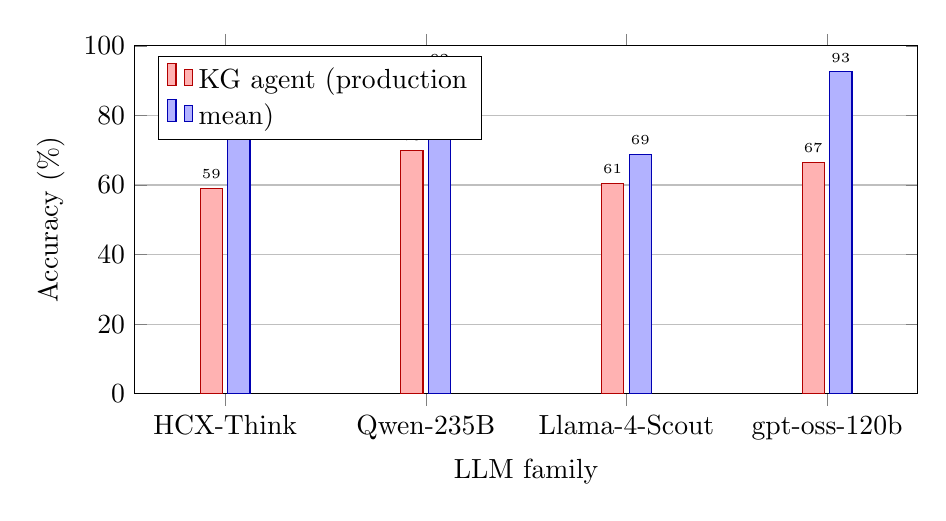
\begin{tikzpicture}
\begin{axis}[
  width=0.95\textwidth,
  height=6cm,
  ybar=2pt,
  bar width=8pt,
  ymin=0, ymax=100,
  ymajorgrids=true,
  ylabel={Accuracy (\%)},
  xlabel={LLM family},
  symbolic x coords={HCX-Think, Qwen-235B, Llama-4-Scout, gpt-oss-120b},
  xtick=data,
  legend pos=north west,
  legend cell align=left,
  enlarge x limits=0.15,
  nodes near coords,
  nodes near coords align={vertical},
  nodes near coords style={font=\tiny},
  every node near coord/.append style={/pgf/number format/.cd, fixed, precision=0},
]
% KG-agent mean = (typedb + neo4j) / 2
\addplot[fill=red!30, draw=red!70!black] coordinates {
  (HCX-Think, 59) (Qwen-235B, 70) (Llama-4-Scout, 60.5) (gpt-oss-120b, 66.5)
};
% In-context mean = (TQL + Cypher + NL + JSONLD) / 4
\addplot[fill=blue!30, draw=blue!70!black] coordinates {
  (HCX-Think, 87.75) (Qwen-235B, 92) (Llama-4-Scout, 68.75) (gpt-oss-120b, 92.5)
};
\legend{KG agent (production, mean), In-context surface form (mean)}
\end{axis}
\end{tikzpicture}
\caption{Production KG-RAG agents (mean of \backendname{typedb} and
\backendname{neo4j}) vs.\ in-context surface-form ablation
(mean of \backendname{C-TQL}, \backendname{C-Cypher}, \backendname{C-NL},
\backendname{C-JSONLD}). The in-context surface forms outperform the
production KG agents in all four LLM families, despite the KG agents
having access to a strictly larger graph (more entities and relations
than the dump). The gap ranges from 8 percentage points
(Llama-4-Scout, where the in-context tier is itself dragged down by KG
syntax familiarity) to 26 percentage points (gpt-oss-120b).}
\label{fig:kg-vs-incontext}
\end{figure}


This is counterintuitive in two ways. First, the KG agents
\emph{strictly} have access to more facts than the in-context dumps:
the production TypeDB and Neo4j stores contain entities that we did
not include in the in-context dumps (career tracks, allowance entities,
12 supplementary clauses, and three additional base-salary tables for
non-comprehensive-planning grades). Second, the KG agents are designed
exactly for multi-hop and multi-key queries — the regime in which the
in-context tiers should struggle most.

To test the gap rigorously we run paired McNemar exact two-sided
binomial tests on discordant pairs (Table~\ref{tab:mcnemar}). Of eight
KG-vs-context comparisons, five are statistically significant at
$p<0.05$ uncorrected, two are borderline ($p=0.052$), and only one
(Qwen-235B \backendname{typedb} vs \backendname{context}) fails to
reject the null. The win counts in the discordant column tell the
story: in HCX the KG agents win at most 5 questions while the context
agent wins 26.

% Table: McNemar paired tests for the main H1 (KG agent vs in-context).
% Exact two-sided binomial test on discordant pairs. n = 100 per cell.
\begin{table}[t]
\centering
\caption{Paired McNemar exact two-sided binomial tests over 100 paired
questions; only discordant pairs contribute to the statistic. Cell
format: ``$a$\,wins -- $b$\,wins'' counts the number of questions on
which only $a$ (resp. only $b$) is correct. Bold marks $p<0.05$.}
\label{tab:mcnemar}
\small
\begin{tabular}{l l c c}
\toprule
LLM & Comparison ($A$ vs $B$) & $A$ wins -- $B$ wins & $p$ \\
\midrule
\multirow{2}{*}{HCX-32B-Think}
 & \backendname{typedb} vs \backendname{context}   & 5 -- 26 & \textbf{0.0002} \\
 & \backendname{neo4j}  vs \backendname{context}   & 4 -- 23 & \textbf{0.0003} \\
\midrule
\multirow{2}{*}{Qwen3-235B}
 & \backendname{typedb} vs \backendname{context}   & 7 -- 14 & 0.189 \\
 & \backendname{neo4j}  vs \backendname{context}   & 5 -- 18 & \textbf{0.011} \\
\midrule
\multirow{2}{*}{Llama-4-Scout}
 & \backendname{typedb} vs \backendname{context}   & 3 -- 23 & \textbf{0.0001} \\
 & \backendname{neo4j}  vs \backendname{context}   & 5 -- 16 & \textbf{0.027} \\
\midrule
\multirow{2}{*}{gpt-oss-120b}
 & \backendname{typedb} vs \backendname{context}   & 8 -- 19 & 0.052 \\
 & \backendname{neo4j}  vs \backendname{context}   & 8 -- 22 & \textbf{0.016} \\
\bottomrule
\end{tabular}
\end{table}


\paragraph{Multiple-testing correction.}
The picture is consistent under family-wise control. Bonferroni
correction at $\alpha/8 = 0.00625$ leaves three comparisons significant
(HCX \backendname{typedb}, HCX \backendname{neo4j}, Llama-4
\backendname{typedb}). Holm--Bonferroni concurs. Benjamini--Hochberg
FDR control at $\alpha=0.05$ yields six significant comparisons,
additionally Qwen \backendname{neo4j} and Llama-4 \backendname{neo4j}.
The headline finding — production KG agents under-performing
in-context tiers — survives the most conservative family-wise
correction in three of four LLM families.

\subsection{The query-generation stage is the bottleneck, not KG expressivity}

The KG agents and the in-context dumps differ in exactly one
operational respect: the KG agents \emph{generate a query} (TypeQL or
Cypher) whose results they then verbalize, while the in-context dumps
hand the full graph directly to the chat model. Since the in-context
dumps preserve the same hyper-relational role-player structure
(C-TQL) or property-graph structure (C-Cypher) that the KG agents
exploit operationally, any drop in KG-agent accuracy must be
attributed to the additional pipeline stages: query authoring, query
execution, and result re-verbalization. The 8--26 percentage-point
gap therefore quantifies the cumulative loss of those stages — the
\emph{query-generation bottleneck}.

\subsection{Closed-book leakage is low}

The \backendname{closed\_book} baselines achieve 9--13\% on the same
100 questions, with a four-LLM mean of 11.25\%. This bounds the
contribution of pre-training memorization to RAG performance: the
75--80 point gap between any RAG-style backend and
\backendname{closed\_book} is genuine retrieval, not regurgitation
of memorized facts.

\subsection{Natural-language summary Pareto-dominates structured surface forms}

Among the in-context tiers, C-NL achieves the highest mean accuracy
(89.8\% across LLMs) at less than half the token cost of the
structured tiers (14K characters vs.\ 26--32K).
Table~\ref{tab:token-cost} and Figure~\ref{fig:pareto} display the
trade-off.

% Table: Surface-form size comparison (token efficiency frontier).
\begin{table}[t]
\centering
\caption{Surface-form size and mean accuracy across four LLM families.
C-NL Pareto-dominates the other in-context tiers: highest mean accuracy
at less than half the token cost.}
\label{tab:token-cost}
\small
\begin{tabular}{l r r}
\toprule
Surface form & Size (chars) & Mean accuracy \\
\midrule
C-MD (production retrieval, chunked) & $\sim$13K & 78.5\% \\
C-TQL (TypeQL insert dump)            & 32{,}436 & 83.3\% \\
C-Cypher (Cypher CREATE dump)         & 32{,}030 & 82.8\% \\
\textbf{C-NL (natural-language summary)} & \textbf{14{,}000} & \textbf{89.8\%} \\
C-JSONLD (nested JSON-LD)             & 26{,}278 & 85.3\% \\
\bottomrule
\end{tabular}
\end{table}

% Figure: Accuracy vs token cost — Pareto frontier shows C-NL dominates.
\begin{figure}[t]
\centering
\begin{tikzpicture}
\begin{axis}[
  width=0.85\textwidth,
  height=6cm,
  xlabel={Surface-form size (characters)},
  ylabel={Mean accuracy across four LLMs (\%)},
  xmin=10000, xmax=35000,
  ymin=75, ymax=95,
  ymajorgrids=true,
  xmajorgrids=true,
  scatter/classes={
    md={mark=triangle*, mark size=4pt, blue!50!black},
    tql={mark=square*, mark size=4pt, red!70!black},
    cy={mark=square*, mark size=4pt, orange!80!black},
    nl={mark=*, mark size=5pt, green!50!black},
    jsonld={mark=square*, mark size=4pt, purple!70!black},
  },
]
\addplot[scatter, only marks, scatter src=explicit symbolic,
  point meta=explicit symbolic, nodes near coords*={\labelname}, every node near coord/.append style={font=\small, anchor=west, xshift=8pt}]
table[meta=label]{
x      y     label    \labelname
13000  78.5  md       C-MD
32436  83.3  tql      C-TQL
32030  82.8  cy       C-Cypher
14000  89.8  nl       C-NL
26278  85.3  jsonld   C-JSONLD
};
\end{axis}
\end{tikzpicture}
\caption{Accuracy versus surface-form size (characters), averaged across
four LLM families. C-NL Pareto-dominates the structured surface forms:
highest mean accuracy at less than half the token cost. C-MD (production
chunked retrieval) under-performs full-graph dumps because retrieval
loses some context; the structured dumps (TQL, Cypher, JSON-LD) gain
nothing for their ~2.3$\times$ token overhead.}
\label{fig:pareto}
\end{figure}


The structured tiers (TQL, Cypher, JSON-LD) bring no accuracy benefit
proportional to their token overhead. The single exception —
gpt-oss-120b on C-TQL at 95\% — does not generalize: Llama-4-Scout
falls to 63\% on the same surface form, dragging down the C-TQL
mean. C-NL is the only surface form that maintains $\geq 83\%$
accuracy across all four LLMs.

\subsection{On Setting A vs.\ Setting B}

A 30-question pilot under \emph{Setting A} — same LLM as chat and
query agent — produced LLM-family-asymmetric KG results: Qwen3-235B
on \backendname{neo4j} jumped +23\,pp from Setting A to Setting B,
while \backendname{typedb} dropped --6\,pp. The asymmetry confirms
that single-LLM measurements conflate KG-backend effects with the
LLM's TypeQL/Cypher syntax familiarity, which is precisely the
mechanism Section~\ref{sec:mechanism} dissects. We therefore use
Setting B (query agent fixed at Qwen3-Coder-30B) as the
production-realistic configuration throughout this paper. Full
Setting A figures appear in Appendix~\ref{sec:appendix}; we report
them transparently rather than as a contrast that flatters the
main result.

\subsection{Multi-key categories: the regime KG agents are designed for}

Restricting to the H1-relevant categories — \texttt{calculation},
\texttt{comparison}, \texttt{multihop\_3key} (42 questions total) —
sharpens the picture: the KG agents range from 47.6\% to 66.7\%
on this subset (mean 57\%) while the in-context tiers reach
57.1\%--100\% (mean 90\%). The regime that hyper-relational KGs are
operationally tailored for is precisely where the in-context
full-graph dumps win largest, with per-LLM multi-key gaps of
17.9, 32.7, 39.9, and 41.7 percentage points (Llama-4-Scout,
Qwen3-235B, HCX-32B-Think, gpt-oss-120b respectively).

\section{Mechanism Findings}\label{sec:mechanism}

The headline result of Section~\ref{sec:results} — that in-context
surface forms beat the production KG agents — leaves open
\emph{which} surface form properties drive the gap. Three mechanism
findings, summarized below, refine the picture.

\subsection{Query-Language Familiarity Dominates LLM-Family Effects}

Three of four LLM families are essentially form-agnostic across the
four in-context tiers. The form-by-form spread is 6 percentage
points for HCX-32B-Think (85--91), 3 for Qwen3-235B (90--93), and
4 for gpt-oss-120b (91--95). Llama-4-Scout is the outlier: a
21-percentage-point spread driven by a steep drop on the structured
tiers (C-TQL 63\%, C-Cypher 62\%, C-JSONLD 67\%) while C-NL holds at
83\%. Figure~\ref{fig:form-sensitivity} visualizes the asymmetry.

% Figure: Llama-4 form sensitivity vs other LLMs.
\begin{figure}[t]
\centering
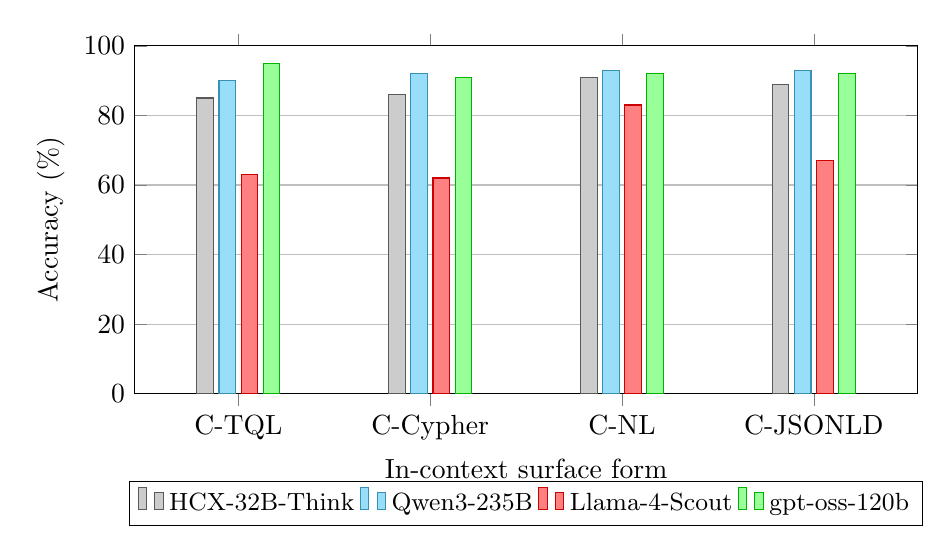
\begin{tikzpicture}
\begin{axis}[
  width=0.95\textwidth,
  height=6cm,
  ybar=2pt,
  bar width=6pt,
  ymin=0, ymax=100,
  ymajorgrids=true,
  ylabel={Accuracy (\%)},
  xlabel={In-context surface form},
  symbolic x coords={C-TQL, C-Cypher, C-NL, C-JSONLD},
  xtick=data,
  legend style={at={(0.5,-0.25)}, anchor=north, legend columns=4, font=\small},
  enlarge x limits=0.18,
]
\addplot[fill=gray!40, draw=gray!70!black] coordinates {
  (C-TQL, 85) (C-Cypher, 86) (C-NL, 91) (C-JSONLD, 89)
};
\addplot[fill=cyan!40, draw=cyan!70!black] coordinates {
  (C-TQL, 90) (C-Cypher, 92) (C-NL, 93) (C-JSONLD, 93)
};
\addplot[fill=red!50, draw=red!80!black] coordinates {
  (C-TQL, 63) (C-Cypher, 62) (C-NL, 83) (C-JSONLD, 67)
};
\addplot[fill=green!40, draw=green!70!black] coordinates {
  (C-TQL, 95) (C-Cypher, 91) (C-NL, 92) (C-JSONLD, 92)
};
\legend{HCX-32B-Think, Qwen3-235B, Llama-4-Scout, gpt-oss-120b}
\end{axis}
\end{tikzpicture}
\caption{In-context surface-form accuracy by LLM family. Three of four
LLMs are essentially form-agnostic (within 8 percentage points across
TQL, Cypher, NL, JSON-LD). Llama-4-Scout exhibits a 21-percentage-point
gap (C-NL 83\% vs.\ C-TQL/Cypher 62--63\%), tracing the bottleneck to
\emph{query-language familiarity in pretraining} rather than the
expressivity of the underlying KG.}
\label{fig:form-sensitivity}
\end{figure}


The asymmetry traces directly to query-language familiarity in the
LLM's pre-training corpus. C-TQL's role-player syntax \texttt{(role1:
\$a, role2: \$b) isa Relation;} appears far less frequently in
public text than Cypher \texttt{CREATE (a)-[:R]->(b)} or JSON-LD,
which is itself less common than English prose. Llama-4-Scout's
weakness on the structured tiers reproduces in production
\backendname{typedb} (56\%), where the agent must in addition
\emph{generate} TQL queries — confirming that the bottleneck is not
the data model but the query-language interface.

\paragraph{Per-category breakdown (Llama-4 C-TQL).}
Within Llama-4's 63\% on C-TQL, the failure modes are not uniform:
single-fact extraction tasks remain strong (\texttt{calculation}
86\%, \texttt{article\_text} 100\%), while cross-reference tasks
collapse (\texttt{comparison} 38\%, \texttt{multihop\_3key} 47\%,
\texttt{aggregation} 50\%, \texttt{negation\_exception} 25\%).
Lookup of one fact survives an unfamiliar syntax; \emph{traversing}
multiple facts under that syntax does not.

\subsection{In-Context KG Underperforms NL on Boundary Inference}

The previous section's mechanism is about \emph{positive}
queries — where the answer exists in the data. A symmetric question
is whether the surface form matters for \emph{negative} queries,
where the correct answer is "no such fact exists." We isolate the
six \texttt{out\_of\_scope} questions: each asks for a
(position, grade), (country, grade), or (allowance) combination
that is provably absent from the regulation tables. For all six
questions the in-context dumps contain enough information to derive
the absence (the position-pay table lists all valid combinations,
the overseas-pay table lists all six countries, and the article-text
prefix defines the closed set of allowances).

% Figure: Out-of-scope category — closed-world boundary inference.
% In-context KG (TQL/Cypher) underperforms NL despite full data coverage.
\begin{figure}[t]
\centering
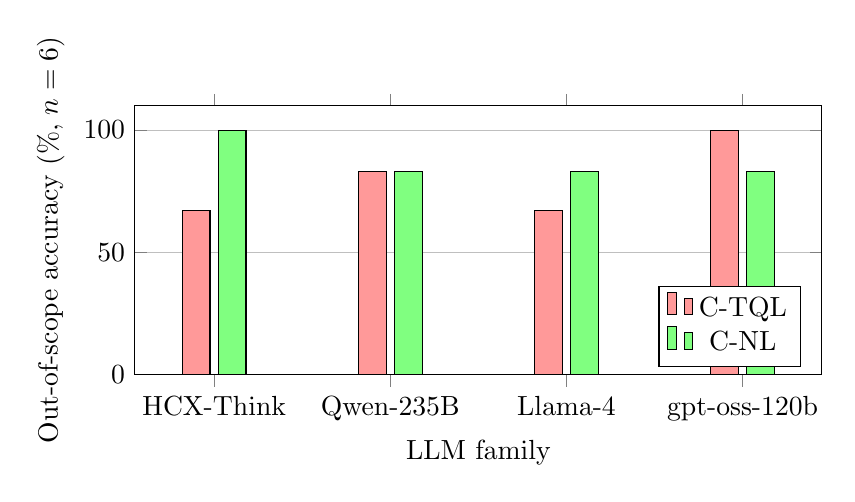
\begin{tikzpicture}
\begin{axis}[
  width=0.85\textwidth,
  height=5cm,
  ybar=3pt,
  bar width=10pt,
  ymin=0, ymax=110,
  ymajorgrids=true,
  ylabel={Out-of-scope accuracy (\%, $n=6$)},
  xlabel={LLM family},
  symbolic x coords={HCX-Think, Qwen-235B, Llama-4, gpt-oss-120b},
  xtick=data,
  legend pos=south east,
  enlarge x limits=0.15,
]
% C-TQL (formal KG)
\addplot[fill=red!40] coordinates {
  (HCX-Think, 67) (Qwen-235B, 83) (Llama-4, 67) (gpt-oss-120b, 100)
};
% C-NL (natural language)
\addplot[fill=green!50] coordinates {
  (HCX-Think, 100) (Qwen-235B, 83) (Llama-4, 83) (gpt-oss-120b, 83)
};
\legend{C-TQL, C-NL}
\end{axis}
\end{tikzpicture}
\caption{Closed-world boundary inference (out-of-scope category, $n=6$).
\textbf{Despite both surface forms containing the same facts}, the
formal KG dump (C-TQL) underperforms natural language (C-NL) on three of
four LLM families. Proving \emph{absence} requires enumeration plus
non-existence verification — a higher cognitive load that compounds with
the lower familiarity of TypeQL syntax. Sample size is small ($n=6$);
this figure is qualitative evidence; per-LLM, per-category breakdowns
are available in the released raw predictions.}
\label{fig:oos}
\end{figure}


Despite full data coverage, the formal KG dumps under-perform
natural language on this category. We attribute this to three
compounding factors:

\begin{enumerate}
\item \textbf{Cognitive load.} A positive lookup requires one
      retrieval. A negative lookup requires \emph{enumerating} all
      candidate facts of the relevant type and verifying that none
      match — a multi-step reasoning chain that is harder under any
      surface form, and especially harder when the syntax is
      unfamiliar.
\item \textbf{Closed-world ambiguity.} A raw KG dump does not signal
      whether absence implies "false" (closed world) or "unknown"
      (open world). The chat model must infer the regime from
      context. Natural-language summary, by contrast, can carry an
      explicit boundary clause — "X is defined only for grades $a$
      and $b$" — verbatim.
\item \textbf{Missing boundary markers.} TypeQL \texttt{insert}
      statements and Cypher \texttt{CREATE} statements are inherently
      assertional: they only express what \emph{is}. There is no
      natural place to assert what \emph{is not}. JSON-LD and
      natural-language summaries have, by contrast, easy linguistic
      affordances for boundary statements.
\end{enumerate}

\subsection{The KG Semantic Paradox}

The two preceding mechanisms compose into what we call the \emph{KG
semantic paradox}. The very strengths that make a KG operationally
valuable — schema-driven structural clarity, explicit role-player
constraints, integrity rules — disappear or invert when the graph is
serialized into an in-context prompt for an LLM. The closed-world
semantics that the operational system relies upon implicitly are
stripped away in raw dumps; the schema constraints are not
reproduced as boundary statements; and the formal query language
that a KG agent could in principle use to express negation
(\texttt{not \{...\};} in TypeQL) is itself the syntactic regime in
which LLMs are weakest. The KG's structural strength becomes its
in-context weakness.

\subsection{Syntax Guides Partially Compensate}

If the bottleneck is query-language familiarity, an
explicit syntax guide should narrow the gap. We test this with
Llama-4-Scout, the model with the largest spread, on C-Cypher (its
weakest formal surface form at 62\%). We prepend a 453-character
syntax primer — three sentences explaining how Cypher's
\texttt{CREATE (var:Label \{prop: value\})-[:REL]->(target)}
notation should be read — and re-run all 100 questions.

\begin{table}[t]
\centering
\caption{Llama-4-Scout on C-Cypher with and without a 453-character
Cypher syntax primer. The guide partially closes the form-sensitivity
gap, with the largest lifts on cross-reference tasks. Out-of-scope
\emph{decreases} (--16.7 pp), suggesting that a syntax guide alone
does not address closed-world boundary inference.}
\label{tab:guide-cypher}
\small
\begin{tabular}{l rrr}
\toprule
Category & C-Cypher & C-Cypher+guide & $\Delta$ \\
\midrule
single\_lookup        & 40.0\% & 60.0\% & $+20.0$ \\
comparison            & 46.2\% & 61.5\% & $+15.4$ \\
aggregation           & 30.0\% & 40.0\% & $+10.0$ \\
calculation           & 92.9\% & 100\%  & $+7.1$  \\
multihop\_3key        & 66.7\% & 73.3\% & $+6.7$  \\
article\_text         & 100\%  & 100\%  & $0$     \\
term\_normalization   & 100\%  & 100\%  & $0$     \\
negation\_exception   & 25.0\% & 25.0\% & $0$     \\
join\_2key            & 60.0\% & 50.0\% & $-10.0$ \\
out\_of\_scope        & 66.7\% & 50.0\% & $-16.7$ \\
\midrule
\textbf{Overall}      & \textbf{62.0\%} & \textbf{67.0\%} & \textbf{$+5.0$} \\
\bottomrule
\end{tabular}
\end{table}

The 5-percentage-point overall lift is non-trivial: it confirms that
syntax familiarity is part of Llama-4's bottleneck, with categories
demanding cross-reference (comparison, single\_lookup,
multihop\_3key) showing the largest individual gains. Tellingly,
\texttt{out\_of\_scope} drops by 16.7 percentage points: a structural
syntax guide is the wrong remedy for closed-world boundary inference.
The two mechanisms are distinct and require distinct interventions.

A 16-percentage-point gap to C-NL (83\%) remains even with the
guide. Syntax familiarity is necessary but not sufficient for closing
the surface-form gap; some additional load — possibly the
cross-reference cognitive cost of formal-syntax reading — persists
beyond what a brief primer can fix.

\paragraph{Guide effectiveness depends on baseline familiarity.}
To probe the limits of the syntax-guide remedy, we repeat the
ablation on C-TQL — the same Llama-4-Scout, the same primer
methodology, a 531-character TypeQL primer explaining N-ary
role-player notation. The result inverts: C-TQL drops from 63\% to
55.8\% (a 7.2-percentage-point regression), with the largest
per-category losses on \texttt{calculation} (--30.2~pp) and
\texttt{join\_2key} (--20.0~pp). Strikingly, the same primer lifts
\texttt{out\_of\_scope} accuracy from 67\% to 100\% (+33.3~pp): the
explicit description of role-player roles seems to prompt the model
to reason about \emph{which} roles are present and absent, but at
the cost of confusing single-fact lookup that was previously working
on syntactic-pattern matching alone.

We read this as evidence that guide remedies are conditional on
baseline syntactic familiarity. Cypher's \texttt{CREATE
(a)-[:R]->(b)} pattern is sufficiently represented in the LLM's
pre-training that a brief primer activates correctly. TypeQL's
N-ary role-player syntax is sufficiently rare that the primer
introduces \emph{new} cognitive load (parsing the guide itself,
re-interpreting prior partial patterns) rather than reinforcing an
existing capability. The implication is that low-familiarity formal
languages may not be repairable from the prompt side at all;
specialized fine-tuning or query-language-aware coder models
(Section~\ref{sec:discussion}, Recommendation~3) are the more
plausible remedy. We treat full coverage of this ablation (four
LLMs $\times$ three structured tiers $\times$ ±guide) as future
work.

\section{Discussion}\label{sec:discussion}

\subsection{KG Infrastructure as Operational Backbone, Not LLM Interface}

Our results suggest a reframing of KG infrastructure value in the
LLM era. The conventional motivation for deploying a hyper-relational
KG in front of an LLM is the expressivity argument: the KG can
faithfully represent N-ary facts and structural constraints that
binary triples or natural language cannot. Our data shows that this
expressivity argument does not transfer to the LLM-facing
interface — given the same facts in-context, all surface forms
including natural language reach $\geq 83\%$ accuracy, with NL the
Pareto winner on accuracy and token cost simultaneously.

The value of KG infrastructure therefore lies elsewhere. We identify
four operational dimensions in which KGs remain critical:

\begin{enumerate}
\item \textbf{Production scalability.} Schema enforcement, integrity
      constraints, concurrency control, and ACID transactions are
      properties of the database backbone, not of any single
      LLM-facing prompt. A KG store provides these for free; an
      LLM-prompt pipeline that holds facts only in JSON files has to
      re-implement them.
\item \textbf{Multi-system source of truth.} A KG can serve a chat
      LLM, a BI dashboard, an audit pipeline, and an internal API
      from a single fact store. The LLM interface is one of many
      consumers; the KG's role is integration substrate.
\item \textbf{Boundary-and-rule encoding.} Schema constraints
      (cardinality, role types, mandatory attributes) and explicit
      negation queries (\texttt{not \{...\};}) let a KG agent reason
      about \emph{absence} in a way an in-context dump cannot. The
      mechanism findings of Section~\ref{sec:mechanism} suggest that
      the largest residual KG advantage — closed-world boundary
      inference — is best exploited via the agent's query interface,
      not the LLM's reading of a raw dump.
\item \textbf{Latent expressivity for stronger query agents.} Today
      the query-generation LLM is the bottleneck. As specialized
      coder LLMs improve at TypeQL, Cypher, and similar domain
      languages, the production KG agent's accuracy is bounded above
      by KG expressivity, not by surface form. The current 30-point
      gap may be closeable from the agent side, not the
      surface-form side.
\end{enumerate}

\subsection{Practical Recommendations for KG-LLM Pipelines}

Our findings yield four concrete recommendations.

\paragraph{Recommendation 1: Add a KG-to-NL conversion layer.} For
in-context QA, structure-preserving NL summary outperforms TypeQL,
Cypher, and JSON-LD on both accuracy and token cost. Generation can
be templated (one sentence per fact) and is fully deterministic
from the source data. Production should ship this layer between the
KG store and the chat LLM, treating the structured surface forms as
debug or audit views rather than the LLM-facing form.

\paragraph{Recommendation 2: Augment NL with explicit boundary
annotations.} The mechanism analysis showed that even NL loses some
out-of-scope accuracy because the dump enumerates only positive
facts. Adding a boundary clause per relation — \emph{"X is defined
only for grades $a$ and $b$; other grades are not in this table"} —
is a deterministic transformation from the schema and should lift
out-of-scope accuracy further. We treat measurement of this lift
as future work.

\paragraph{Recommendation 3: Specialize the query-generation LLM.}
Setting B's query-model fix to Qwen3-Coder partially explains why
Llama-4-Scout's KG agent (56\%) is worse than its in-context tier
(63\%): the chat-side syntax weakness compounds with the absent
syntax-aware specialization on the query side. As the available
specialized coder models grow more competent at KG query languages,
we expect the production-agent / in-context gap to narrow from the
agent side. Practitioners should track coder-LLM benchmarks for
TypeQL and Cypher as a leading indicator.

\paragraph{Recommendation 4: Treat KG as backbone, not interface.}
The four dimensions in Section~7.1 motivate keeping the KG store as
the source of truth and the integration substrate. The LLM
interface above it should be a thin NL-summary layer with optional
agent fall-through for queries the summary cannot answer (e.g.,
counts, filters, multi-hop traversals beyond the summary template).
This inverts the common architecture in which the KG agent is
\emph{primary} and a context document is the fall-back.

\subsection{Scope: Fact-Bounded KGs in the 32K-Token Regime}

A natural objection is that our findings apply only when the entire
KG fits in the LLM context, and thus cannot generalize to KGs serving
Web-scale or multi-million-fact use cases. We accept this scope but
argue the relevant population is larger than it first appears.
Regulations, internal policies, benefits schedules, clinical
guidelines, organizational handbooks, compliance frameworks, and many
enterprise knowledge bases serialize to a few megabytes of structured
facts — well inside the 32K--200K token windows of current LLMs. For
\emph{this} substantial class of domains, our results are directly
applicable: production teams currently invest in KG-agent
infrastructure where the cheaper, more accurate path is an in-context
NL summary. The argument for KG infrastructure shifts from "in-context
limits" (where it does not hold for fact-bounded KGs) to the four
operational dimensions in \S7.1. For Web-scale or open-domain KGs, the
retrieval problem is different and our findings do not extend; we
treat this as an explicit boundary.

\subsection{Relation to Counterintuitive H1}

The pre-experiment hypothesis — "even a maximally preprocessed
context-RAG cannot match a hyper-relational KG agent on multi-key
queries" — is rejected by our data ($p<0.05$ in 5/8 KG-vs-context
comparisons, all in the opposite direction). The data
\emph{does} support a different counterintuitive claim: that the
production KG agent's query-generation stage, not the KG's
expressivity, is the dominant accuracy determinant in this
deployment regime. This new claim shares the original's
counterintuitive framing — practitioners typically assume that more
structure leads to better LLM downstream performance — while being
directly evidenced by the surface-form ablation.

\section{Limitations and Future Work}\label{sec:limits}

\paragraph{Single domain, single language.}
The evaluation domain is one Korean public-sector compensation
regulation. Generalization to other regulatory domains, to English
or other languages, and to private-sector enterprise data is left to
future work. Two of the four LLM families (HCX-32B-Think, Qwen3-235B)
have substantial Korean pre-training; the other two (Llama-4-Scout,
gpt-oss-120b) are predominantly English. Form-sensitivity findings
should be interpreted within this LLM-family mix.

\paragraph{Sample size.}
The 100-question evaluation set is balanced across ten categories
but yields modest per-category power: the
\texttt{out\_of\_scope} category in particular has $n=6$, so the
boundary-inference finding (Section~6.2) is qualitative. Scaling
to 1{,}000+ questions, with explicit balance toward boundary and
multi-key categories, is the highest-priority follow-on.

\paragraph{Production-agent specifics.}
The KG-agent results are tied to one specific production
implementation (LangGraph ReAct with three-attempt retries). A
different agent — for example, a graph-aware retrieval-then-rerank
pipeline like GraphRAG \citep{edge2024graphrag} or a
PageRank-driven retriever like HippoRAG
\citep{gutierrez2024hipporag} — could close some of the
30-percentage-point gap. We do not include such external baselines
in the present paper; doing so is a critical next step before
generalizing the "query-generation bottleneck" claim beyond
ReAct-style agents.

\paragraph{Surface forms covered.}
We test four surface forms (TQL, Cypher, NL, JSON-LD). Other
surface forms — RDF/Turtle, the OpenIE-style triple format used by
some retrieval pipelines, and graph-summary text from GraphRAG —
remain untested. The Pareto-optimality claim for NL is strictly
within the four tested forms.

\paragraph{Schema coverage of in-context dumps.}
The in-context dumps cover the core fact tables (salary, position
pay, differential, cap, wage peak, bonus rate, overseas pay,
starting step, six categories of position) but omit several
production-side entities: career-track entities, allowance entities,
12 supplementary clauses (부칙) with their override relations, and
salary tables for non-comprehensive-planning grades (GA/CL/PO).
The KG agents have full graph access; the in-context tiers do not.
The asymmetry favors the KG agents, which makes the observed in-
context-tier advantage \emph{stronger} than the headline numbers
suggest.

\paragraph{Single non-reasoning configuration.}
All chat LLMs run in non-reasoning mode (no thinking-flag
activation, no chain-of-thought scaffolding). Whether reasoning
modes — particularly for HCX-32B-Think and gpt-oss-120b — would
narrow the KG-agent gap is a natural ablation we leave as future
work.

\paragraph{Closed-book leakage.}
Closed-book accuracy is uniformly $\leq 13\%$, indicating low
pre-training memorization of these specific Korean compensation
facts. However, the four LLMs have heterogeneous training cutoffs
and language coverage, and we do not control for the precise
publication date of training corpora. Replication on data published
\emph{after} all model cutoffs would strengthen the claim that the
RAG accuracy gap is genuinely retrieval, not memorization.

\paragraph{Future work.}
Beyond the items above, we identify three directions: (i) systematic
guide ablation across all four LLMs and three formal surface forms,
(ii) explicit-boundary NL variants with measured lift on
\texttt{out\_of\_scope} and \texttt{negation\_exception}, and (iii)
multi-domain extension covering at least one English-language
regulatory corpus to test cross-language transfer of the
form-sensitivity mechanism.

\section{Conclusion}\label{sec:conclusion}

We have shown, on a 100-question Korean public-sector regulation
benchmark with four LLM families, that the production KG-RAG
agents — built on TypeDB v3 and Neo4j — underperform an in-context
surface-form ablation of the \emph{same} knowledge graph by
8--26 percentage points (paired McNemar $p<0.05$ in 5 of 8
KG-vs-context comparisons). The result holds despite the agents
having strictly more data and being deployed for exactly the
multi-key reasoning regime they appear designed to dominate.

The bottleneck is the query-generation stage of the KG agent, not
the expressivity of the KG itself: an in-context dump that
preserves the same hyper-relational role-player structure reaches
83--95\% accuracy. Within that in-context regime, natural-language
summary Pareto-dominates the formal surface forms (TypeQL, Cypher,
JSON-LD) on both accuracy and token cost, and the only LLM family
sensitive to structural surface-form (Llama-4-Scout) reveals a
secondary mechanism: pre-training query-language familiarity that
syntax guides only partly compensate for. A third mechanism — the
\emph{KG semantic paradox} — shows that the very structural clarity
that makes a KG operationally valuable disappears when serialized,
hurting closed-world boundary inference relative to natural
language.

We argue that KG infrastructure should be treated as the
\emph{operational backbone} of the system — schema enforcement,
multi-system integration, query-agent improvement potential — and
that its LLM-facing layer should be a structure-preserving
natural-language summary, augmented with explicit boundary
annotations. The reframing is constructive rather than dismissive:
KGs remain irreplaceable for the operational dimensions, and the
gap between the production KG agent and the in-context tier is a
roadmap for stronger query-generation models, not a verdict on
KG expressivity.

\paragraph{Future work.}
We outline three priorities in Section~\ref{sec:limits}:
multi-domain replication beyond Korean public-sector regulation,
explicit-boundary NL variants with quantified lift on the
out-of-scope category, and external-baseline comparison
(GraphRAG, HippoRAG) on the same evaluation set.

\paragraph{Reproducibility.}
The evaluation set, scorer, runner, and surface-form dump
generators are released at
\url{https://github.com/shezgone/bok-comp-eval}. Three of the four
LLM families used (Qwen3-235B, Llama-4-Scout, gpt-oss-120b) are
open-weight; replication on their HuggingFace checkpoints
reproduces the in-context-tier numbers.


\bibliographystyle{plainnat}
\bibliography{refs}

\appendix
\section{Appendix}\label{sec:appendix}

\subsection{Setting A vs.\ Setting B (Pilot)}

In an early 30-question pilot we measured the KG agents under
\emph{Setting A}, in which a single LLM played both reasoner and
query-author roles, before fixing the query agent at
Qwen3-Coder-30B (Setting B). Setting A produced strongly asymmetric
results across LLM families that confounded the headline KG-vs-
context comparison:

\begin{itemize}
\item Qwen3-235B-Instruct on \backendname{typedb}: 83\% in
      Setting A, 77\% in Setting B (--6 pp; the larger general
      model authored TQL more fluently than the smaller coder).
\item Qwen3-235B-Instruct on \backendname{neo4j}: 60\% in
      Setting A, 83\% in Setting B (+23 pp; Cypher is more
      represented in Qwen-Coder's training).
\item HCX on \backendname{typedb}: 60\% in Setting A, 63\% in
      Setting B (+3 pp).
\end{itemize}

The asymmetry confirms that single-LLM measurements conflate KG-
backend effects with query-language familiarity. Setting B isolates
the chat-model variable; all main-paper numbers are Setting B.

\subsection{Surface-Form Sample Excerpts}

For reference, the same fact —"a Grade-1 employee in the position
\emph{부서장(가)} (Department Head Type-1) has an annual
position-pay of 18{,}192{,}000 KRW"— is rendered in the four
in-context tiers as follows.

\paragraph{C-TQL.}
\begin{verbatim}
$g1 isa 직급, has 직급명 "1급", has 직급서열 1;
$p_bsg_a isa 직위, has 직위명 "부서장(가)";
$pp_P01_1급 isa 직책급기준, has 직책급액 18192000;
(해당직급:$g1, 해당직위:$p_bsg_a, 적용기준:$pp_P01_1급) isa 직책급결정;
\end{verbatim}

\paragraph{C-Cypher.}
\begin{verbatim}
CREATE (g1:JobGrade {name: "1급", order: 1});
CREATE (p_bsg_a:Position {code: "P01", name: "부서장(가)"});
CREATE (pp_P01_1급:PositionPay {annual_amount: 18192000});
CREATE (g1)-[:HAS_POSITION_PAY]->(pp_P01_1급);
CREATE (p_bsg_a)-[:HAS_POSITION_PAY]->(pp_P01_1급);
\end{verbatim}

\paragraph{C-NL.}
\begin{quote}
부서장(가) 직위에 있는 1급 직원의 연간 직책급은 18,192,000원이다. \\[2pt]
\textit{[gloss: A Grade-1 employee in the position
부서장(가) (Department Head Type-1) has an annual position-pay of
18{,}192{,}000 KRW.]}
\end{quote}

\paragraph{C-JSONLD.}
\begin{verbatim}
{
  "직책급": [
    {"직위코드": "P01", "직위명": "부서장(가)",
     "직급": "1급", "연간직책급": 18192000}
  ]
}
\end{verbatim}

\subsection{Cypher Syntax Guide (Section 6.4)}

The 453-character Cypher primer prepended to C-Cypher+guide for the
Llama-4-Scout ablation:

\begin{quote}\small
\textit{[The Cypher dump represents a Neo4j property graph. Read
\texttt{CREATE (var:Label \{prop: value, ...\})} as defining a node
of the given label with properties; read
\texttt{CREATE (a)-[:REL\_TYPE \{prop: value\}]->(b)} as a directed
binary relationship from \texttt{a} to \texttt{b} with optional
edge properties. Same variables refer to the same node across
statements. Multi-arity facts (e.g., position pay with both
position and grade) are flattened by introducing intermediate
nodes connected to all participants.]}
\end{quote}


\end{document}
